\part{Resultados}
\chapter[Resultados]{Análise Estatística de Usabilidade}
Nesta seção, são apresentados, de maneira concisa, os resultados principais derivados da interação dos \textit{usuários testes} com a plataforma em estudo. Estes resultados foram meticulosamente adquiridos por intermédio do \textit{PostHog}, uma ferramenta de análise de fluxo de usuários.

O PostHog, implementado em TypeScript, desempenha uma função central no gerenciamento de dados, permitindo a captura de eventos desde o \textit{login} de um usuário até o acompanhamento de ações específicas dentro da plataforma online, inclusive a gravação de sessões de usuário em formato de vídeo. Sua integração complementa as demais ferramentas empregadas na construção da plataforma para Terapia Comunitária Integrativa(TCI) online.

A coleta automática de eventos pelo \textit{PostHog} se inicia com a visualização de páginas, abrangendo elementos como o URL dos eventos e se estendendo para ações específicas como cliques, alterações em entradas ou submissões associadas a diversas \textit{tags} personalizáveis. É necessário destacar que o \textit{PostHog} não captura os dados sensíveis do usuário, concentrando-se exclusivamente na coleta de informações relacionadas à usabilidade dentro da plataforma online, com foco especial na definição do tipo de usuário.

Para além do acompanhamento do \textit{front-end}, o \textit{PostHog} revela-se como uma ferramenta multifacetada, também enviando eventos durante atividades no \textit{back-end} ou no início de fluxos de trabalho. Este recurso permite análises em tempo real mesmo durante as fases iniciais de desenvolvimento, ampliando sua utilidade para além da esfera do usuário final. A condução de análises estatísticas robustas propicia uma compreensão aprofundada dos padrões comportamentais dos usuários, desempenhando um papel crucial no aprimoramento contínuo da plataforma para sessões de TCI online.

\section{Dados Obtidos e Análise Estatística de Usabilidade}

A decisão de implementar a captura automática na plataforma por meio do \textit{PostHog} foi motivada por sua configuração ágil, ampla cobertura, eliminação da necessidade de adição manual de eventos personalizados e a vantagem de ser uma solução com ótimo retorno na versão gratuita.

Dentro do contexto do \textit{PostHog}, um evento desempenha um papel central, representando uma ação única executada por um usuário em um momento específico. Os eventos armazenados, não podem ser alterados, garantindo a integridade e confiabilidade dos dados coletados.

As ferramentas de análise essências no \textit{PostHog} são as Ações e \textit{Insights}. Na prática, uma ação simplifica a criação de novos eventos ao filtrar e combinar uma ou mais ações, proporcionando simplicidade nas análises e facilitando a geração de \textit{insights}.

Para a obtenção de dados de usabilidade, foi adotado uma abordagem colaborativa, promovendo convites para voluntários atuarem como \textit{\textbf{usuários testes}} por meio de grupos em redes sociais. Dos 60 voluntários manifestamente interessados, mais de 48\% se cadastraram e acessaram a plataforma no período compreendido entre 24 de novembro e 03 de dezembro de 2023.

No processo de obtenção de dados, fez-se uso dos cinco tipos fundamentais de \textit{insights} fornecidos pelo PostHog: Tendências, Funis, Retenção, Caminhos do Usuário e Aderência. Todos os dados foram gerados pelo \textit{PostHog} e cuidadosamente filtrados considerando os \textit{insights} pertinentes ao período de teste, e estão apresentados de maneira detalhada a seguir: [Inserir os dados apresentados].
\begin{enumerate}
    \item\textbf{Análise de Produto}
    \begin{enumerate}
        \item\textit{\textbf{Dispositivos Utilizados}}\\
 Este gráfico mostra quais dispositivos os usuários únicos mais usaram no período estipulado.
\begin{figure}[!ht]
    \centering
    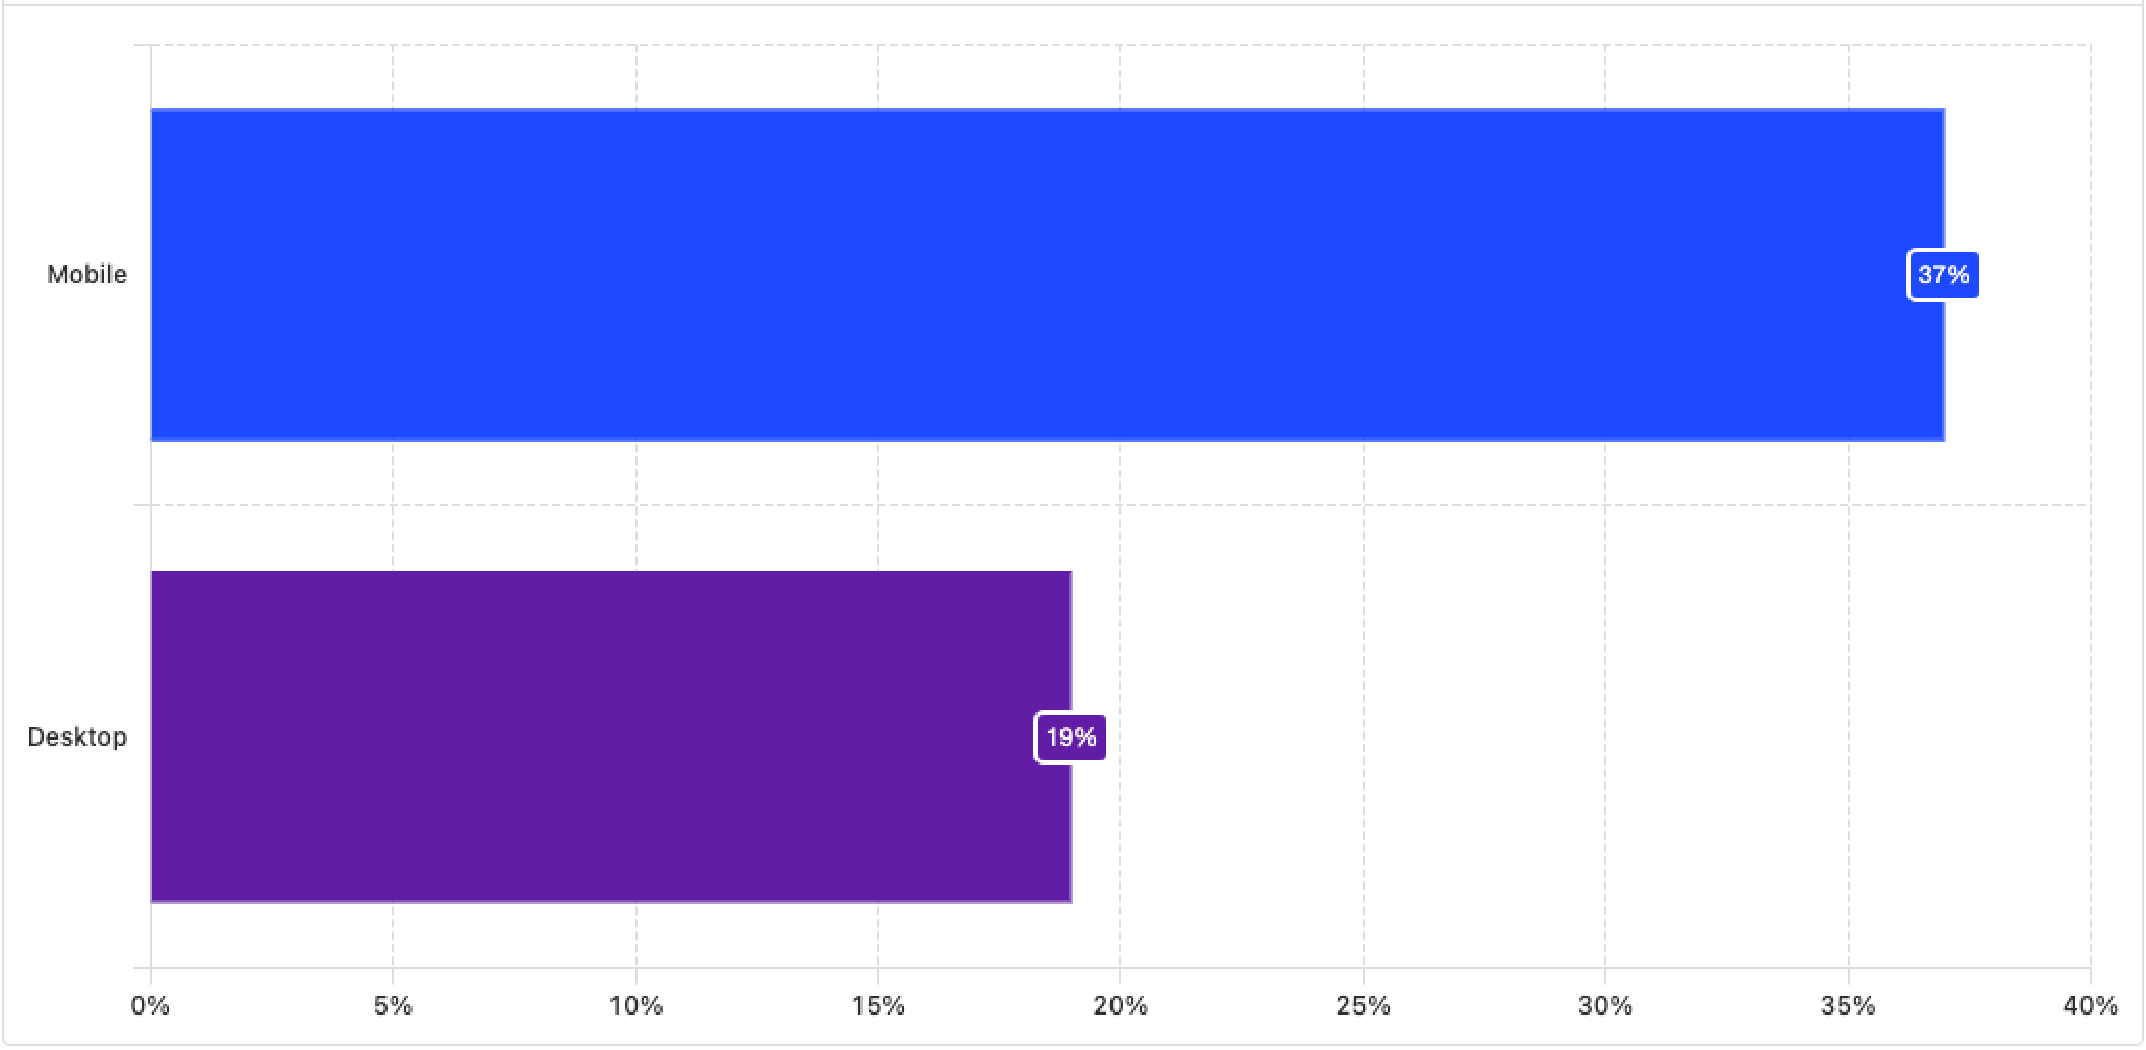
\includegraphics[scale=0.45]{latex/figuras/disp.pdf}
    \label{disp}
    \caption[Dispositivos Utilizados]{Indicadores de Dispositivos Utilizado pelos Usuários}
    \label{fig:enter-label}
\end{figure}\\
 Esses dados são importantes para que possa garantir que está desenvolvendo a plataforma para os dispositivos principais dos usuários de forma correta.

\item\textit{\textbf{Tamanho da Tela}}\\
 Este gráfico exibe a altura de tela mais comum entre usuários únicos.\\
\begin{figure}[!ht]
    \centering
    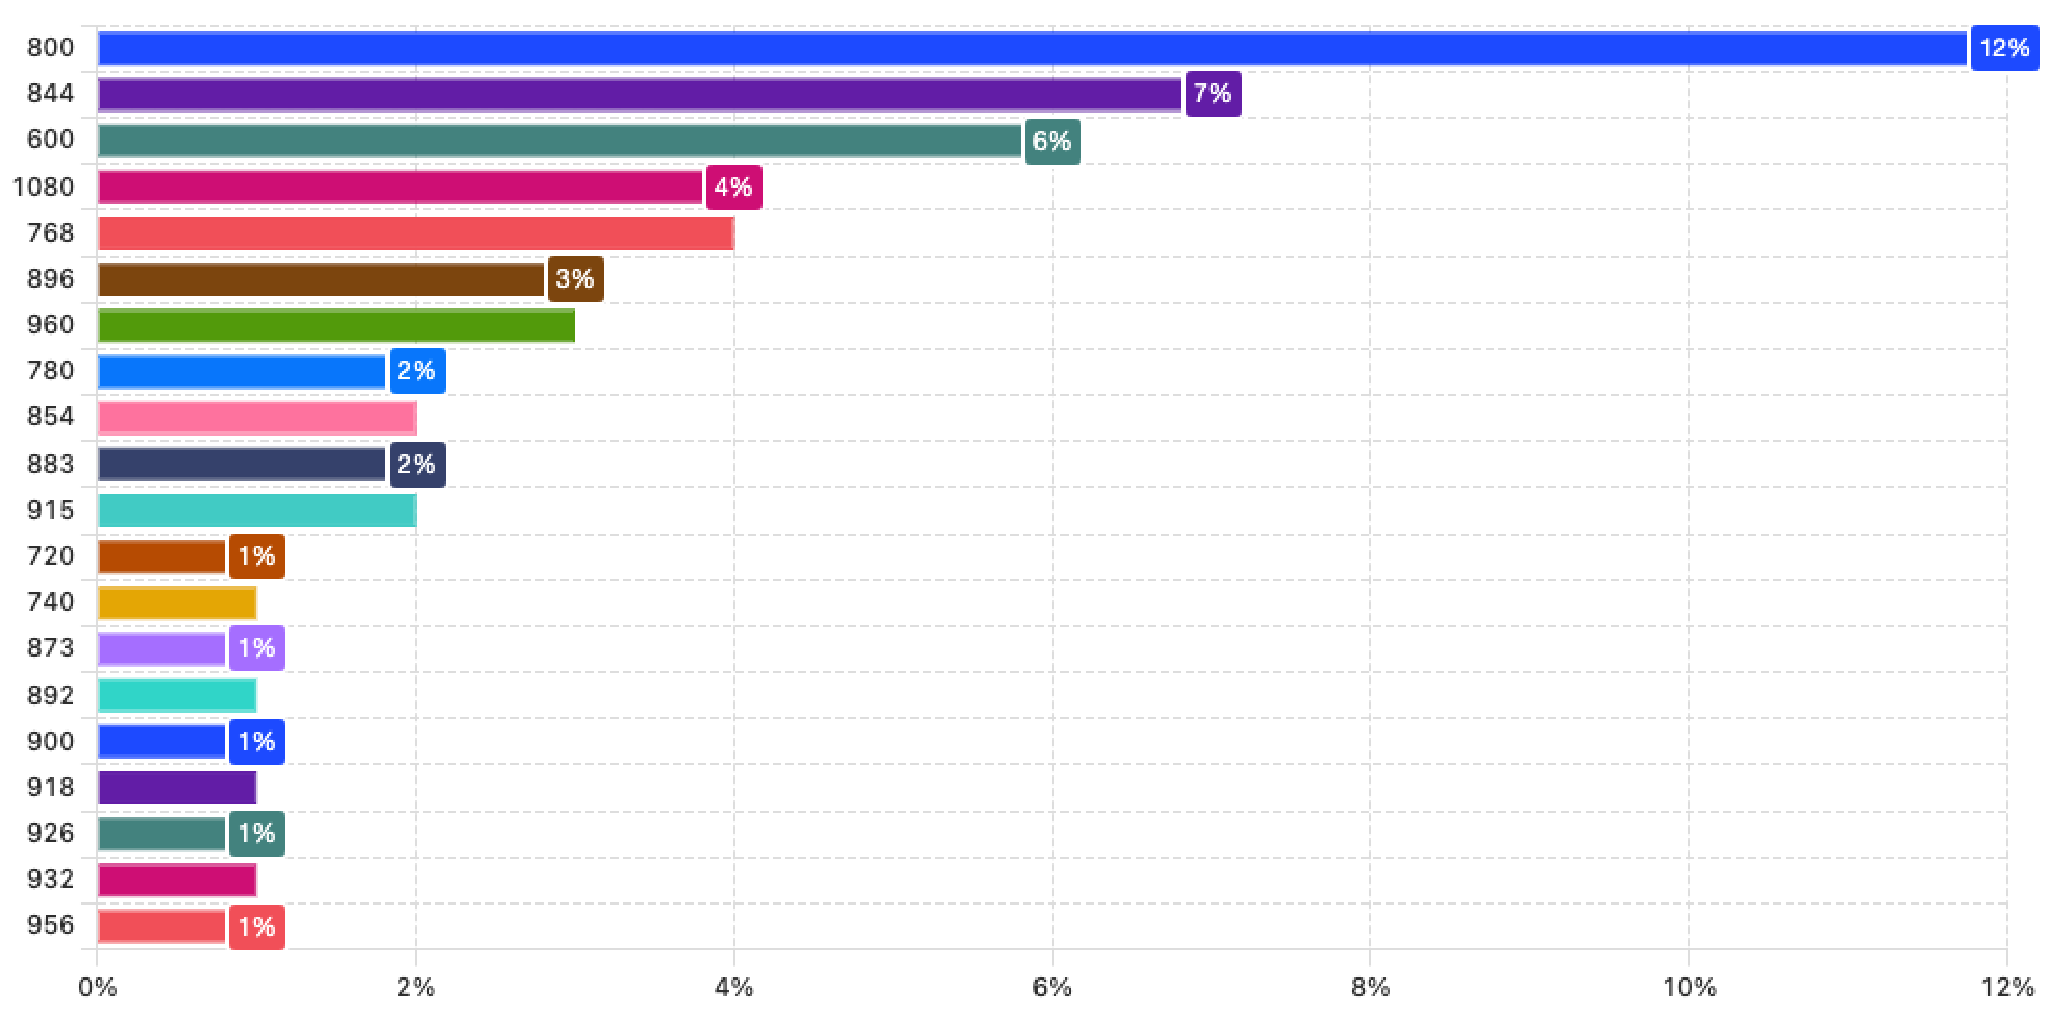
\includegraphics[scale=0.45]{latex/figuras/tela.pdf}
    \label{tela}
    \caption[Tamanho da Tela]{Indicadores do Tamanho da Tela dos Usuários}
    \label{fig:enter-label}
\end{figure}\\
Com essa informação, torna-se viável implementar melhorias no design da plataforma, adaptando o conteúdo aos espaços disponíveis e proporcionando uma experiência mais otimizada para os usuários.
 
\item\textit{\textbf{Funil de Visualização de Página}}\\
 Este funil ilustra o número de usuários que concluíram visualizações de páginas, categorizados por diferentes navegadores. Os dados abrangem todos os acessos à plataforma, sem distinção individual dos usuários, considerando todas as utilizações, independentemente do número de logins realizados pelos usuários.\\
 
\begin{figure}[!ht]
    \centering
    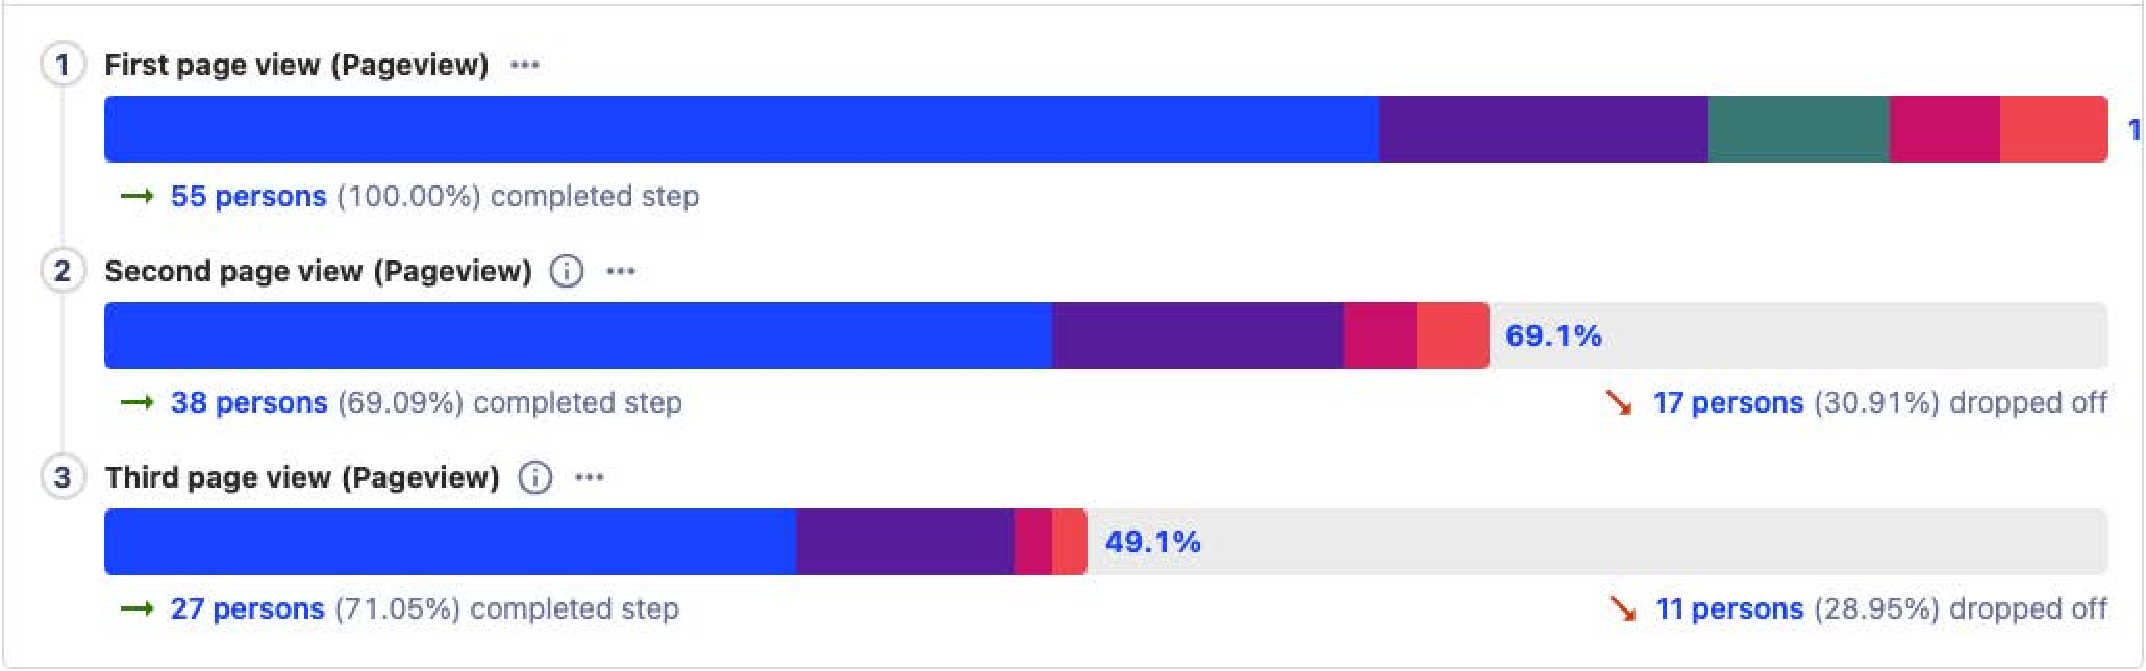
\includegraphics[scale=0.45]{latex/figuras/page.pdf}
    \label{page}
    \caption[Funil de Visualização]{Indicadores de Visualização de Página por Navegador}
    \label{fig:enter-label}
\end{figure}
\textbf{\textbf{Legenda de Cores:}} Google Chrome → azul; Mobile Safari → roxo;\\Empty String → verde; Samsung Internet → rosa pink; Chrome iOS → laranja;\\

Com esses dados, torna-se possível analisar o percurso dos usuários e identificar possíveis pontos de gargalo que levam ao abandono repentino da utilização da plataforma.

\item\textit{\textbf{Fluxo de Usabilidade}}\\
Este trajeto ilustra os sete percursos mais frequentes adotados pelos usuários, iniciando na visualização da página inicial e avançando por três estágios que se ramificam nos perfis. A extensão de um caminho indica sua frequência, sendo as áreas em vermelho indicativas de abandonos abruptos.

\begin{figure}[!ht]
    \centering
    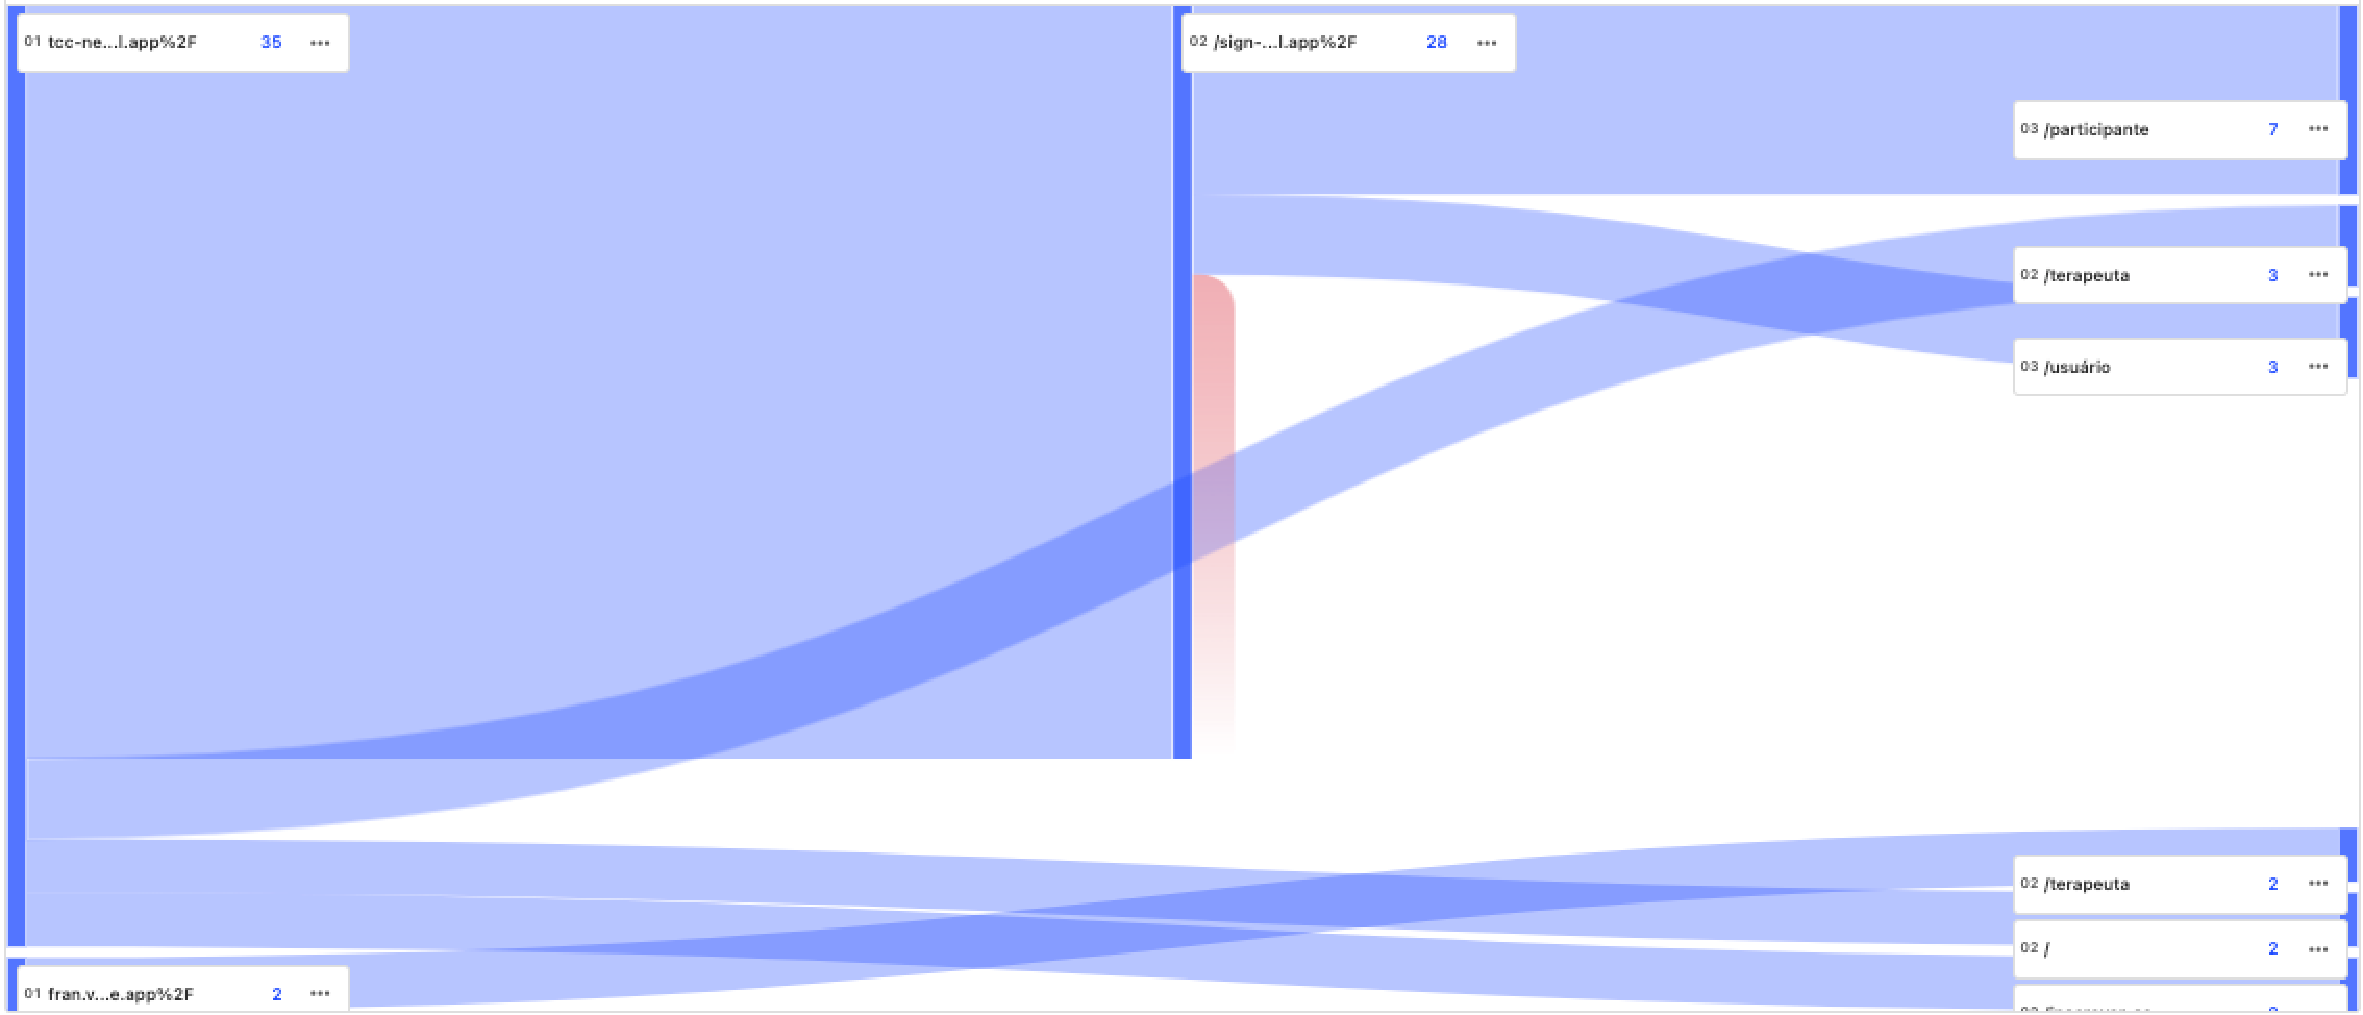
\includegraphics[scale=0.35]{latex/figuras/fluxouso.pdf}
    \label{fluxouso}
    \caption[Fluxo de Usabilidade]{Indicadores de Fluxo de Usabilidade}
    \label{fig:enter-label}
\end{figure}

Esta análise é particularmente valiosa para identificar onde os usuários podem se desorientar e compreender os destinos mais populares.
\end{enumerate}
 
 
\item\textbf{Pesquisa de Usuário}
\begin{enumerate}
    \item\textit{\textbf{Localização Geográfica dos Usuários}}
Este gráfico ilustra a origem de todas as visualizações de página realizadas por usuários distintos.\pagebreak

\begin{figure}[!ht]
    \centering
    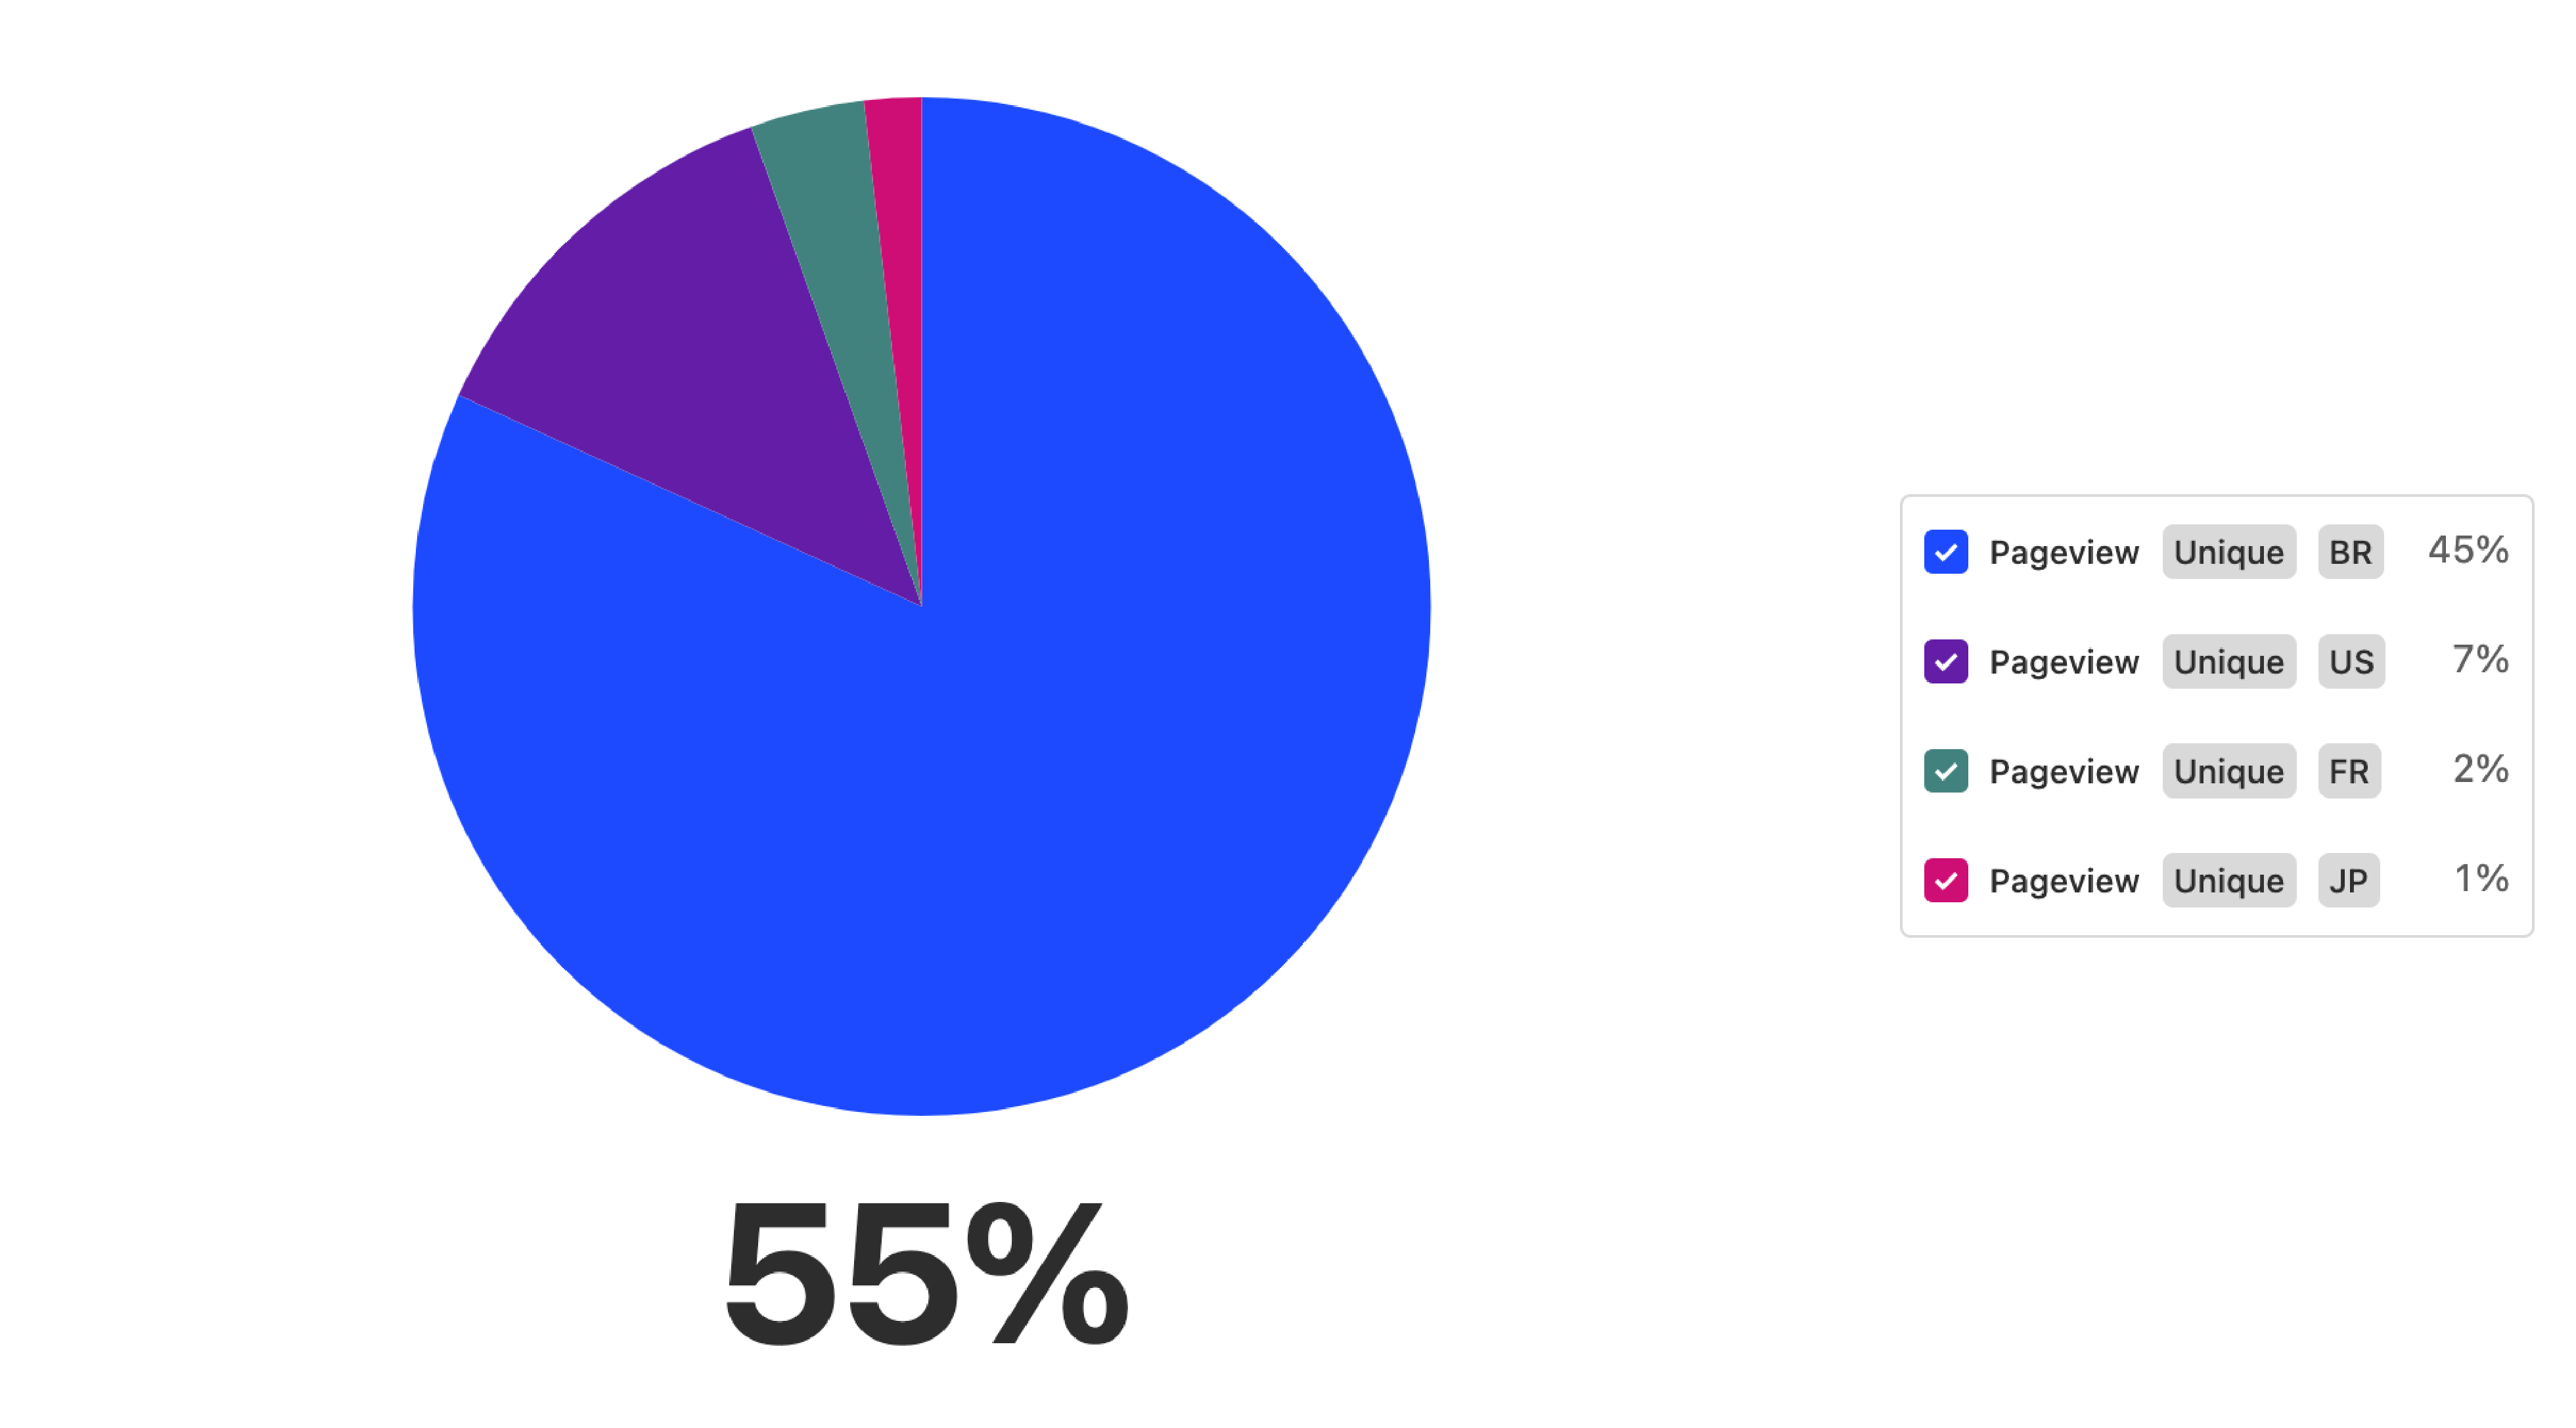
\includegraphics[scale=0.25]{latex/figuras/local.pdf}
    \label{local}
    \caption[Localização Geográfica]{Indicadores de Localização Geográfica dos Usuários}
    \label{fig:enter-label}
\end{figure}

Com essas informações, torna-se viável compreender a procedência dos usuários, sendo de suma importância para avaliar o impacto geográfico gerado pelas sessões de terapia comunitária online.

\item\textit{\textbf{Frustrações de Usabilidade}}\\
Este gráfico evidencia as páginas em que os usuários apresentaram maior persistência ao clicar, seja em botões, menus suspensos, áreas não interativas ou durante a espera pelo carregamento de componentes.

\begin{figure}[!ht]
    \centering
    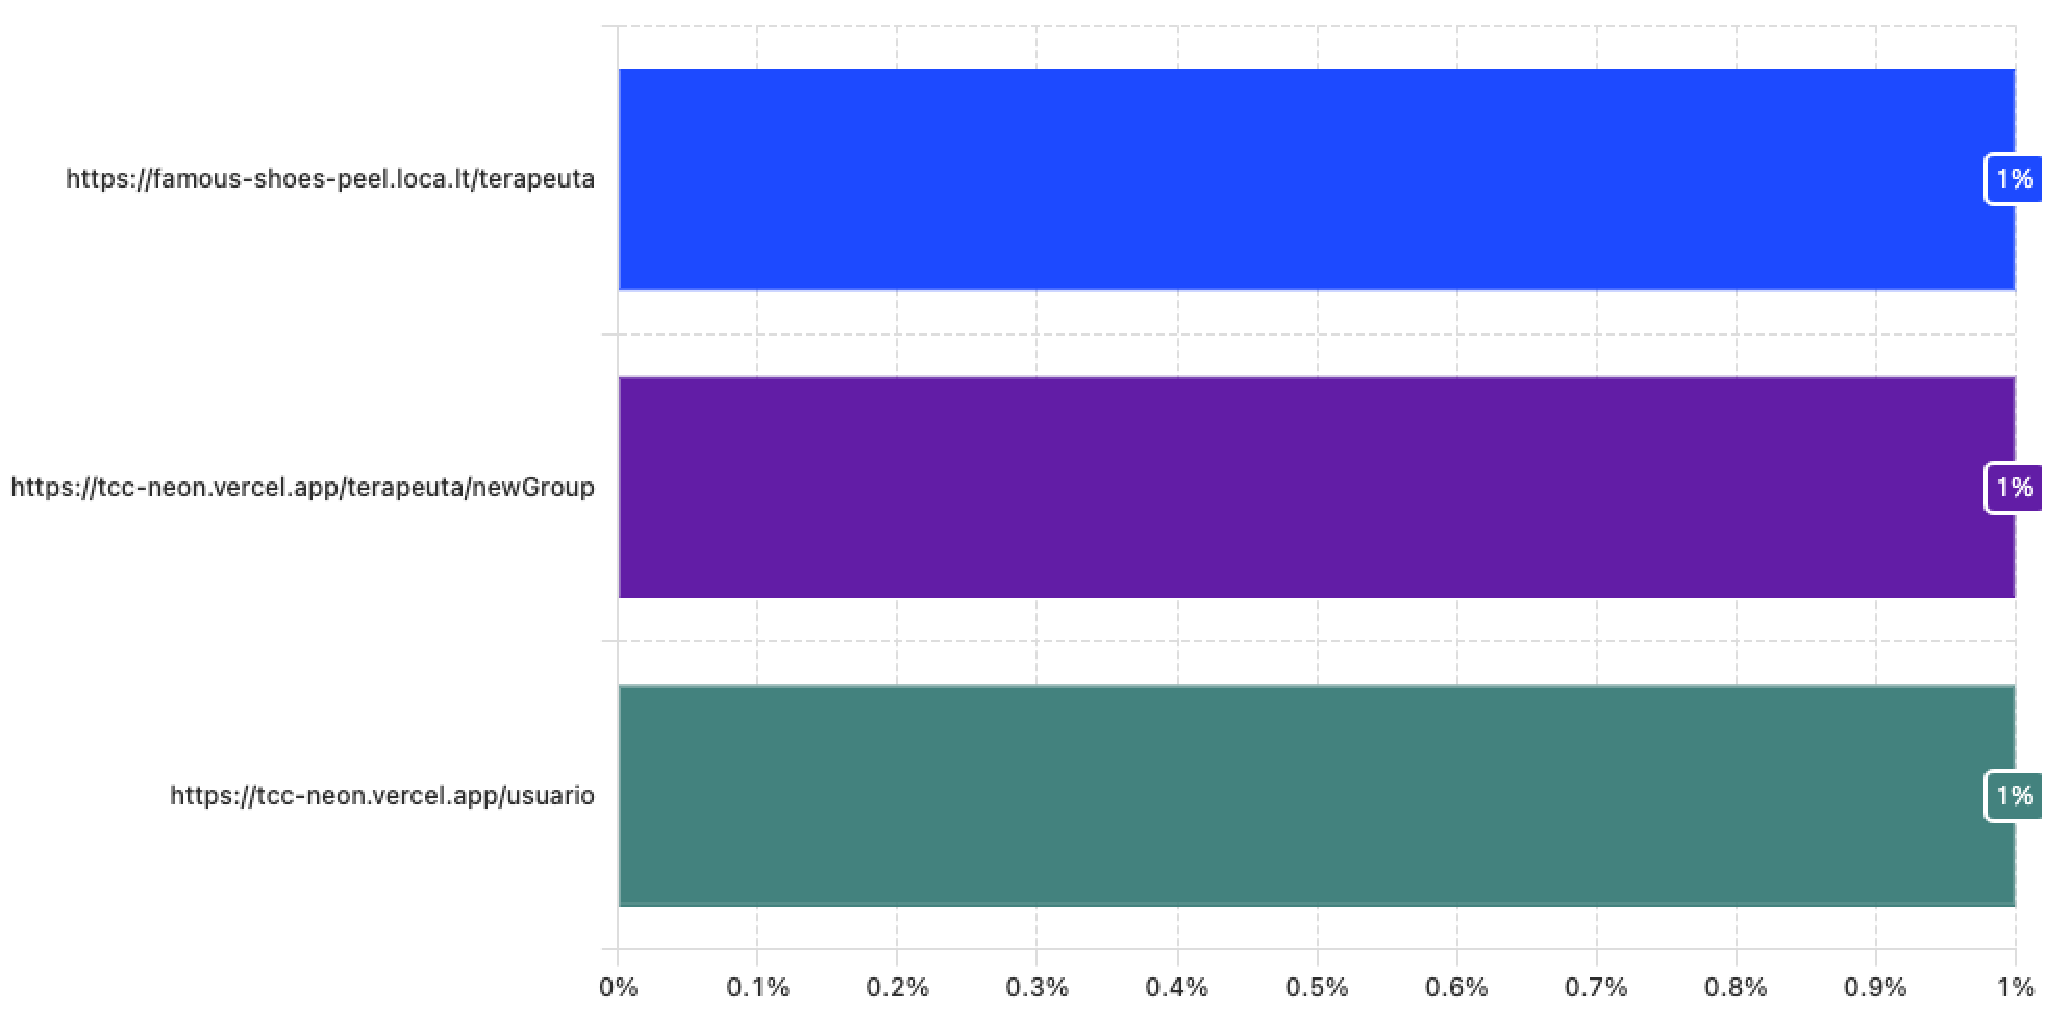
\includegraphics[scale=0.4]{latex/figuras/clique.pdf}
    \label{clique}
    \caption[Frustrações de Usabilidade]{Indicadores de Frustrações no Uso da Plataforma}
    \label{fig:enter-label}
\end{figure}

Esta análise pode revelar-se proveitosa na identificação de áreas na plataforma em que os usuários enfrentam frustrações significativas, abrindo espaço para implementação de melhorias com o intuito de tornar a plataforma mais responsiva e intuitiva.
 
\item\textit{\textbf{Indicadores de Crescimento}}\\
Nessa métrica, torna-se visualmente acessível observar a distribuição semanal dos usuários, classificados como novos (representados em azul), recorrentes (indicados em verde), ressuscitados (apresentados em roxo) e inativos (destacados em vermelho).

\begin{figure}[!ht]
    \centering
    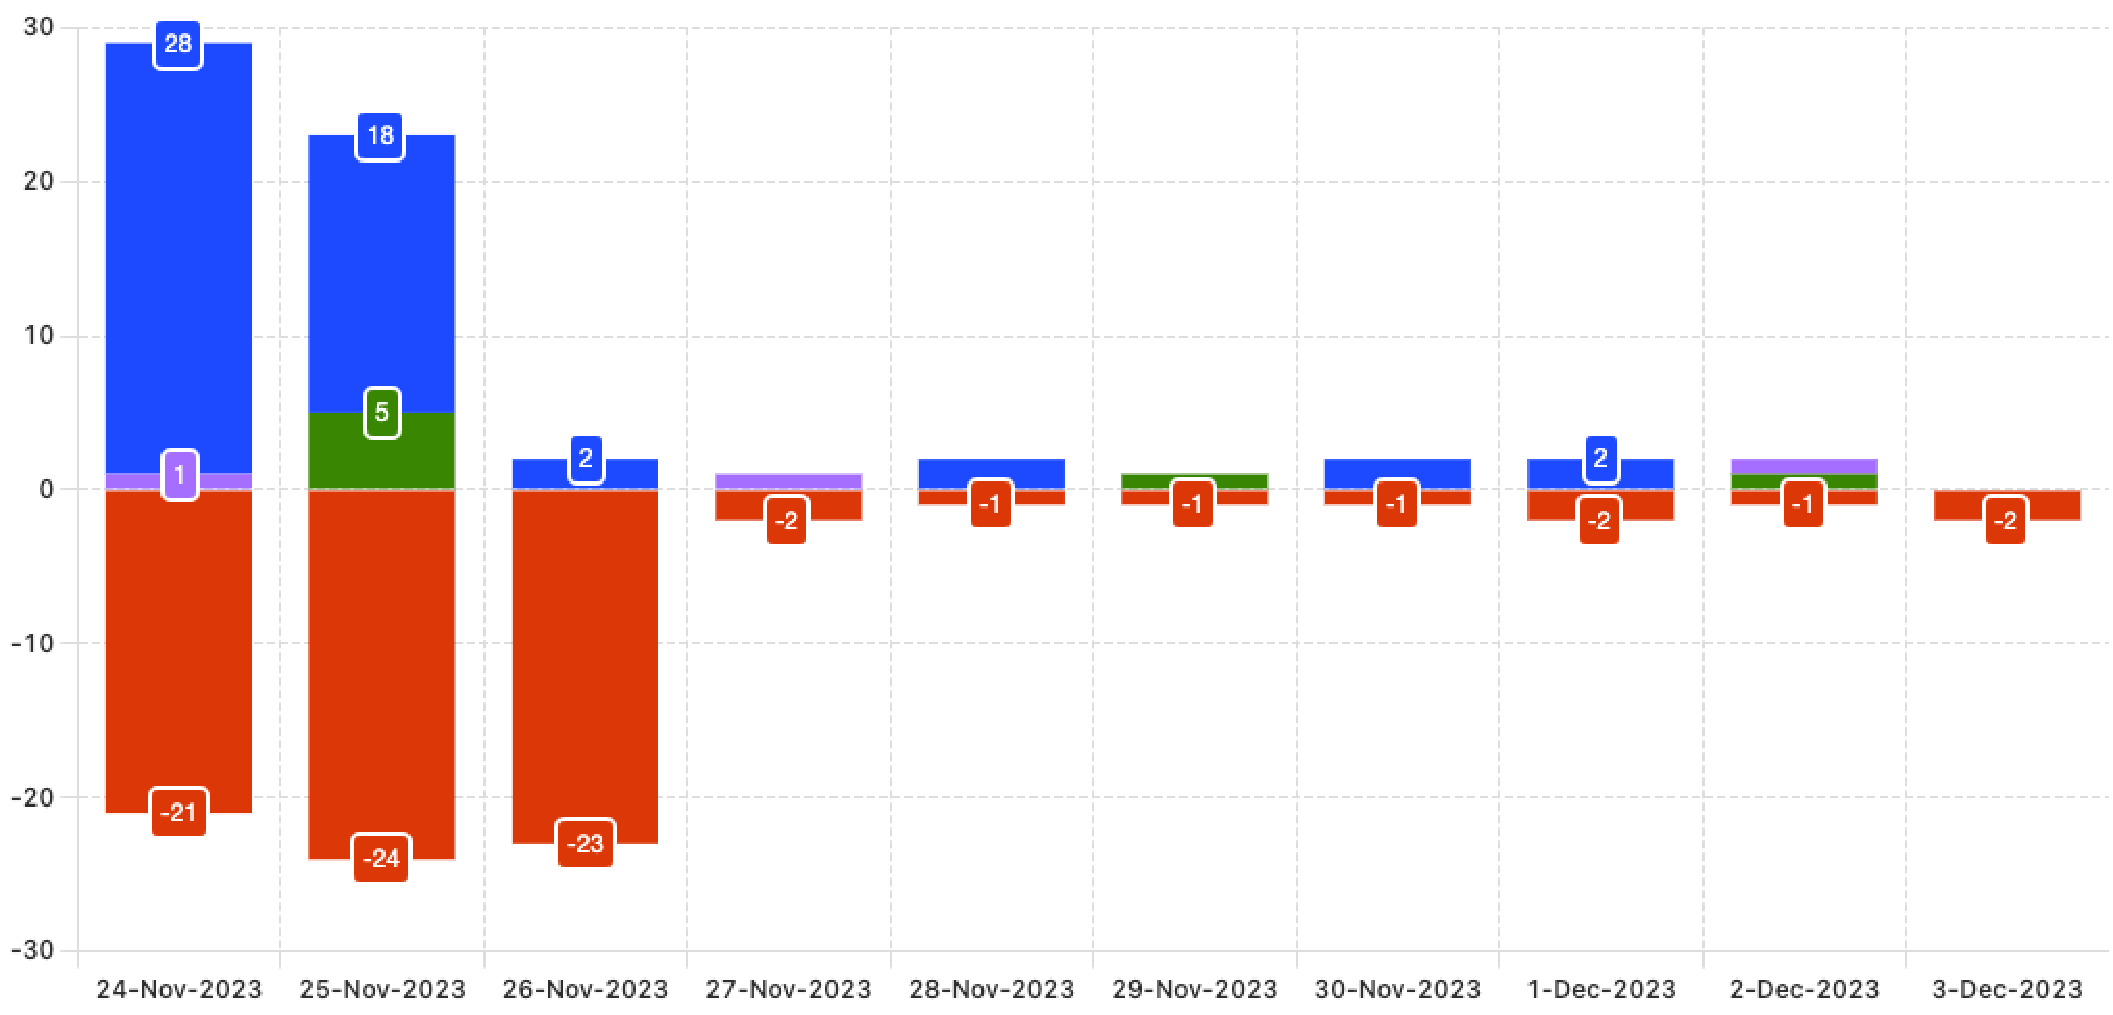
\includegraphics[scale=0.4]{latex/figuras/cresce.pdf}
    \label{cresce}
    \caption[Indicadores de Crescimento]{Indicadores de Crescimento do Uso da Plataforma}
    \label{fig:enter-label}
\end{figure}
 
Com base nestes dados, é factível mensurar o crescimento e a popularidade da plataforma, proporcionando a oportunidade de aprimorá-la tanto em atratividade quanto em eficiência, visando a permanência de todos dos usuários como recorrentes.
\end{enumerate}

\end{enumerate}

O \textit{PostHog} disponibiliza uma ampla variedade de tipos de dados passíveis de extração. No entanto, neste contexto, foram apresentadas apenas as métricas consideradas relevantes para a análise preliminar da utilização da versão inicial de uma plataforma para gerenciamento se sessões online de Terapia Comunitária Integrativa. Através das informações fornecidas, foi possível analisar os padrões de usabilidade dos voluntários designados como \textit\textbf{{usuários testes}} nesta fase, proporcionando uma visão antecipada do impacto em cenários de uso real.
 


\section{Identificação e resolução de problemas}
O PostHog desempenha um papel crucial ao capturar automaticamente eventos do usuário na plataforma de Terapia Comunitária Integrativa (TCI) online. Além de integrar o rastreamento ao produto, a ferramenta envia eventos adicionais em situações específicas, permitindo a inclusão de propriedades customizadas em um evento e garantindo consistência ao longo do tempo.

A capacidade de captura de eventos do PostHog abrange tanto o front-end quanto o back-end, garantindo máxima confiabilidade e flexibilidade na análise de dados para identificação de bugs e aprimoramento da usabilidade.

Essa abordagem abrangente não apenas assegura a entrega confiável de eventos originados no servidor, mas também proporciona dados seguros ao buscar informações diretamente do banco de dados ou de outros serviços que ainda não estão disponíveis no frontend. O PostHog desempenha um papel crucial na identificação e resolução eficaz de problemas na plataforma.

Na sequência, problemas encontrados e as soluções de contorno adotadas: 
[INSERIR BUGS JIRA]


 
 
 
 
 
 % PostHog captura automaticamente eventos do usuário durante o uso dentro da plataforma de TCI online. Além de integrar o rastreamento ao produto, envia eventos adicionais para quando ocorrerem coisas específicas e que não são comuns ao que foi proposto na plataforma. com isso é possível enviar propriedades customizadas de um evento e manter os eventos consistentes ao longo do tempo.
 

 % A ferramenta de analise Posthog, captura eventos de backend  rastreando o servidor, além do front-end. Isso garante máxima confiabilidade e maior flexibilidade ao analisar os dados, o que pode levar a identificação de bugs e outros problemas de usabilidade.
 
 % Isso garante entrega mais confiável, de como esses eventos se originam no seu servidor e dados mais confiáveis, ao fazer buscas de informações atualizadas diretamente do banco de dados ou dos outros serviços, que não estão disponíveis no frontend ainda.
 

% \section{Melhorias e otimizações realizadas}

% houveram algumas sugestao de possíveis melhorias pelos "usuarios testes"


% A utilização de quadros Kanban, no Jira, baseado em fluxo, ofereceu uma oportunidade de desenvolver o que já estava funcionando bem e gradualmente fazer as melhorias e correçoes necessarias e também sugeridas pelos "usuarios teste".  Garantindo assim a entrega de uma plataforma de qualidade, com uma experiência fluida e eficaz para os usuários finais.com a 